\documentclass{beamer}
\usepackage{amsmath}
\usepackage{gvv}

\title{Question 1.4.15}
\author{AI25BTECH11040 - Vivaan Parashar}
\date{\today}

\begin{document}

\frame{\titlepage}

\begin{frame}
    \frametitle{Question: }
    The point which divides the line segment joining the points $\mathbf{P}(7, -6)$ and $\mathbf{Q}(3, 4)$ in the ratio $1 : 2$ internally lies in which quadrant?
\end{frame}

\begin{frame}
    \frametitle{Solution: }
    The point $\vec{C}$ that divides points $\vec{P}$ and $\vec{Q}$ in the ratio $l : m$ is
    \begin{align}
        \vec{C} = \frac{m\vec{P} + l\vec{Q}}{l+m}\
    \end{align}
    $\therefore$ The point $\vec{R}$ dividing $\vec{P}$ and $\vec{Q}$ in the ratio $1:2$ is
    \begin{align}
        \vec{R} = \frac{2\cdot\vec{P}+1\cdot\vec{Q}}{1+2} \\
        \vec{R} = \myvec{\frac{17}{3}                     \\ -\frac{8}{3}}
    \end{align}
    Clearly this point lies in the 4$^\text{th}$ quadrant.
\end{frame}

\begin{frame}
    \frametitle{Plot: }
    \begin{figure}
        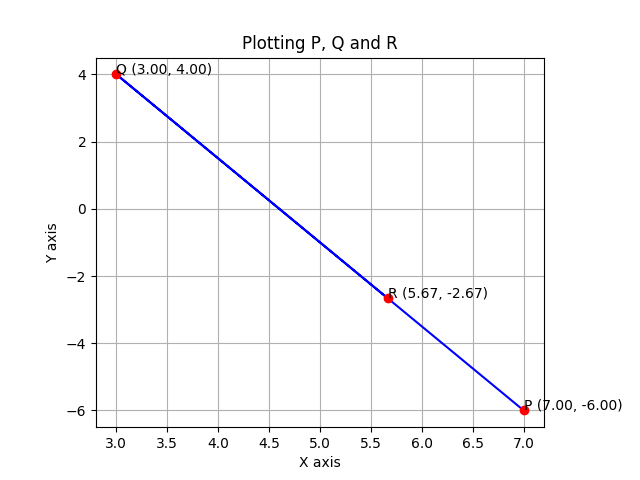
\includegraphics[scale=0.5]{figs/plot.png}
    \end{figure}
\end{frame}

\end{document}
